% Options for packages loaded elsewhere
\PassOptionsToPackage{unicode}{hyperref}
\PassOptionsToPackage{hyphens}{url}
%
\documentclass[
  english,
  ,man,floatsintext]{apa6}
\usepackage{lmodern}
\usepackage{amssymb,amsmath}
\usepackage{ifxetex,ifluatex}
\ifnum 0\ifxetex 1\fi\ifluatex 1\fi=0 % if pdftex
  \usepackage[T1]{fontenc}
  \usepackage[utf8]{inputenc}
  \usepackage{textcomp} % provide euro and other symbols
\else % if luatex or xetex
  \usepackage{unicode-math}
  \defaultfontfeatures{Scale=MatchLowercase}
  \defaultfontfeatures[\rmfamily]{Ligatures=TeX,Scale=1}
\fi
% Use upquote if available, for straight quotes in verbatim environments
\IfFileExists{upquote.sty}{\usepackage{upquote}}{}
\IfFileExists{microtype.sty}{% use microtype if available
  \usepackage[]{microtype}
  \UseMicrotypeSet[protrusion]{basicmath} % disable protrusion for tt fonts
}{}
\makeatletter
\@ifundefined{KOMAClassName}{% if non-KOMA class
  \IfFileExists{parskip.sty}{%
    \usepackage{parskip}
  }{% else
    \setlength{\parindent}{0pt}
    \setlength{\parskip}{6pt plus 2pt minus 1pt}}
}{% if KOMA class
  \KOMAoptions{parskip=half}}
\makeatother
\usepackage{xcolor}
\IfFileExists{xurl.sty}{\usepackage{xurl}}{} % add URL line breaks if available
\IfFileExists{bookmark.sty}{\usepackage{bookmark}}{\usepackage{hyperref}}
\hypersetup{
  pdftitle={The Development of Color Terms in Shipibo-Konibo Children},
  pdfauthor={Danielle Kellier*1, Martin Fortier*2, Maria Fernández Flecha3, \& Michael C. Frank4},
  pdflang={en-EN},
  pdfkeywords={keywords},
  hidelinks,
  pdfcreator={LaTeX via pandoc}}
\urlstyle{same} % disable monospaced font for URLs
\usepackage{graphicx,grffile}
\makeatletter
\def\maxwidth{\ifdim\Gin@nat@width>\linewidth\linewidth\else\Gin@nat@width\fi}
\def\maxheight{\ifdim\Gin@nat@height>\textheight\textheight\else\Gin@nat@height\fi}
\makeatother
% Scale images if necessary, so that they will not overflow the page
% margins by default, and it is still possible to overwrite the defaults
% using explicit options in \includegraphics[width, height, ...]{}
\setkeys{Gin}{width=\maxwidth,height=\maxheight,keepaspectratio}
% Set default figure placement to htbp
\makeatletter
\def\fps@figure{htbp}
\makeatother
\setlength{\emergencystretch}{3em} % prevent overfull lines
\providecommand{\tightlist}{%
  \setlength{\itemsep}{0pt}\setlength{\parskip}{0pt}}
\setcounter{secnumdepth}{-\maxdimen} % remove section numbering
% Make \paragraph and \subparagraph free-standing
\ifx\paragraph\undefined\else
  \let\oldparagraph\paragraph
  \renewcommand{\paragraph}[1]{\oldparagraph{#1}\mbox{}}
\fi
\ifx\subparagraph\undefined\else
  \let\oldsubparagraph\subparagraph
  \renewcommand{\subparagraph}[1]{\oldsubparagraph{#1}\mbox{}}
\fi
% Manuscript styling
\usepackage{upgreek}
\captionsetup{font=singlespacing,justification=justified}

% Table formatting
\usepackage{longtable}
\usepackage{lscape}
% \usepackage[counterclockwise]{rotating}   % Landscape page setup for large tables
\usepackage{multirow}		% Table styling
\usepackage{tabularx}		% Control Column width
\usepackage[flushleft]{threeparttable}	% Allows for three part tables with a specified notes section
\usepackage{threeparttablex}            % Lets threeparttable work with longtable

% Create new environments so endfloat can handle them
% \newenvironment{ltable}
%   {\begin{landscape}\begin{center}\begin{threeparttable}}
%   {\end{threeparttable}\end{center}\end{landscape}}
\newenvironment{lltable}{\begin{landscape}\begin{center}\begin{ThreePartTable}}{\end{ThreePartTable}\end{center}\end{landscape}}

% Enables adjusting longtable caption width to table width
% Solution found at http://golatex.de/longtable-mit-caption-so-breit-wie-die-tabelle-t15767.html
\makeatletter
\newcommand\LastLTentrywidth{1em}
\newlength\longtablewidth
\setlength{\longtablewidth}{1in}
\newcommand{\getlongtablewidth}{\begingroup \ifcsname LT@\roman{LT@tables}\endcsname \global\longtablewidth=0pt \renewcommand{\LT@entry}[2]{\global\advance\longtablewidth by ##2\relax\gdef\LastLTentrywidth{##2}}\@nameuse{LT@\roman{LT@tables}} \fi \endgroup}

% \setlength{\parindent}{0.5in}
% \setlength{\parskip}{0pt plus 0pt minus 0pt}

% \usepackage{etoolbox}
\makeatletter
\patchcmd{\HyOrg@maketitle}
  {\section{\normalfont\normalsize\abstractname}}
  {\section*{\normalfont\normalsize\abstractname}}
  {}{\typeout{Failed to patch abstract.}}
\patchcmd{\HyOrg@maketitle}
  {\section{\protect\normalfont{\@title}}}
  {\section*{\protect\normalfont{\@title}}}
  {}{\typeout{Failed to patch title.}}
\makeatother
\shorttitle{Color Terms in Shipibo-Konibo Children}
\keywords{keywords\newline\indent Word count: X}
\usepackage{lineno}

\linenumbers
\usepackage{csquotes}
\ifxetex
  % Load polyglossia as late as possible: uses bidi with RTL langages (e.g. Hebrew, Arabic)
  \usepackage{polyglossia}
  \setmainlanguage[]{english}
\else
  \usepackage[shorthands=off,main=english]{babel}
\fi

\title{The Development of Color Terms in Shipibo-Konibo Children}
\author{Danielle Kellier*\textsuperscript{1}, Martin Fortier*\textsuperscript{2}, Maria Fernández Flecha\textsuperscript{3}, \& Michael C. Frank\textsuperscript{4}}
\date{}


\affiliation{\vspace{0.5cm}\textsuperscript{1} University of Pennsylvania\\\textsuperscript{2} PSL Research University\\\textsuperscript{3} Pontificia Universidad Católica del Perú\\\textsuperscript{4} Stanford University}

\abstract{
Enter abstract here. Each new line herein must be indented, like this line.
}



\begin{document}
\maketitle

\hypertarget{introduction}{%
\section{Introduction}\label{introduction}}

Color language is where language and perception meet. Terms like \emph{blue} or \emph{red} draw boundary lines across a perceptually continuous space. In English, there are 11 high frequency basic color terms (BCTs), but this color categorization is not universal. For instance, Russian speakers use two distinct words to describe the colors light blue (\enquote{goluboy}) and dark blue (\enquote{siniy}); and some languages have as few as two words (e.g., the Jalé people only have terms for ``light'' and ``dark''; Berlin \& Kay, 1969). Why do languages vary in their color systems? One emerging consensus is that languages categorize the color spectrum in different ways in part due to functional demands (Gibson et al., 2017): both smaller and larger color systems are relatively optimal for suiting different communicative needs (Regier, Kay, \& Khetarpal, 2007; Zaslavsky, Kemp, Tishby, \& Regier, 2018).

Learnability is hypothesized to be one contributor to this cross-linguistic diversity (Chater \& Christiansen, 2010; Culbertson, Smolensky, \& Legendre, 2012). In the domain of color, some color systems may be easier to learn for children than others, or children may show inductive biases that shape color vocabulary. But the actual acquisition of color terms -- while relatively well-studied in English (e.g., Sandhofer \& Smith, 1999; Wagner, Dobkins, \& Barner, 2013) -- is extremely under-studied across other populations. Berlin \& Kay's seminal World Color Survey (WCS; Kay, Berlin, Maffin, Merrifield, \& Cook, 2009) presented adult speakers of over 100 languages with differently colored chips and asked them to produce a label, characterizing the space of color vocabulary in a range of written and unwritten languages. The WCS is an invaluable resource for the cross-linguistic study of color vocabulary, but no comparable resource exists for cross-cultural studies of how this vocabulary is learned across childhood.

In the current project, our goals were (1) to characterize color term knowledge in an indigenous population previously studied by the WCS, the Shipibo-Konibo (SK), and then (2) to build on this foundation to characterize the developmental trajectory of color language acquisition in a group of children raised learning Shipibo-Konibo, outside of the WEIRD (Western Educated Industrialized Rich Democratic) populations that are over-represented in behavioral science (Henrich, Heine, \& Norenzayan, 2010; Nielsen, Haun, Kärtner, \& Legare, 2017). In the remainder of the introduction, we review color vocabulary development in children, and then we turn to reviewing what is currently known about color terms in Latin American varieties of Spanish, such as Mexican, Colombian, and Bolivian Spanish, and in some Amazonian languages, such as Candoshi, Pirahã, and Shipibo Konibo. These two literatures set the stage for our own study.

\hypertarget{the-development-of-color-vocabulary}{%
\subsection{The Development of Color Vocabulary}\label{the-development-of-color-vocabulary}}

To adult speakers, colors are extremely salient attributes of the perceptual world; even when color is seemingly task-irrelevant, we mention it (e.g., Sedivy, 2003). It is quite surprising then that children often struggle to master color vocabulary. As reviewed by H.Bornstein (1985), it has long been noted that color vocabulary is learned quite late in development, with observations by Darwin, Bateman, Nagel, and others attesting to individual children's delays in the correct use of color terms well into middle childhood; several diarists report 5 - 8 year olds with limited mastery of basic level color terms. These observations are surprising in light of the body of infant research that suggests that infants' color \emph{discrimination} abilities are relatively well-developed by the end of the first year of life (for review see e.g., Dobson \& Teller, 1978). The age at which color words are learned has been shifting over the past hundred years, however, at least for English-speaking children. H.Bornstein (1985) documents substantial decreases in the age at which many children master their colors, citing four years as an age at which most children are proficient. In fact, this age may have even decreased further in the last thirty years, judging from recent studies (Wagner et al., 2013; Wagner, Jergens, \& Barner, 2018). What makes color words hard to learn, and why are they getting easier?

One prominent account of what makes color word learning difficult is that children may not recognize that color words pick out the perceptual dimension of hue at all (Bartlett, 1977; Sandhofer \& Smith, 1999), and that once they do they then rapidly map colors correctly onto the appropriate hues. This account nicely explains the observation that there is often a period during which children will produce an inappropriate color word when asked \enquote{what color is this?} -- they know that color words go together and answer a particular question, they just don't know which color is which. A further point of parsimony for this account is that infants' color boundaries are not all that different in their placement from those of adults; thus, presumably the mapping task they face -- from words to hues -- is not all that difficult, once they recognize the dimension that they are attempting to map (Bornstein, Kessen, \& Weiskopf, 1976; Franklin, Pilling, \& Davies, 2005).

On the other hand, when children's mapping errors are examined in detail, they show more systematicity than would be predicted by this account. In particular, Wagner et al. (2013) show that children who may not have full mastery of the color lexicon nevertheless use colors in ways that are more consistent with overextension than with ignorance of the dimensional mapping -- for example, using \enquote{blue} to refer to \emph{blue} and \emph{green} hues (which are close together in color space). These overextensions are reminiscent of overextensions of noun meaning that have been documented in early word learning, for example calling a horse \enquote{dog} (Clark, 1973). The order of acquisition for color word meanings in this study was well-predicted by the frequency and perceptual salience of color categories (Yurovsky, Wagner, Barner, \& Frank, 2015), further supporting the view that color categories are learned gradually from perceptual experiences rather than all at once. Finally, both behavioral and eye-tracking evidence suggests that children show earlier comprehension than production for color words (Sandhofer \& Smith, 1999; Wagner et al., 2018). And in eye-tracking tasks, comprehension also shows evidence of perceptual overextensions, such that children fixate perceptually close distractor colors more than far distractors (Wagner et al., 2018). In sum, although attention to the dimension of hue may be one difficult component of color word learning, but systematic mapping of words to particular regions of perceptual space is likely another.

So why are these processes getting easier -- or at least occurring earlier in development -- for English-learning children? There are at least two obvious, plausible reasons that occur to us. The first is the increasing prevalence of manufactured toys for children that vary exclusively in color (e.g., sets of plastic blocks of different colors) (Gibson et al., 2017). Such objects provide perfect contrastive input for mapping: if one is called \enquote{blue} and the other is not, such input implicates pragmatically that \enquote{blue} is an informative term (Clark, 1987; Frank \& Goodman, 2014). The second is a cultural landscape for parents and early educators that presupposes color words are an important part of early childhood education practices, and as such should be taught explicitly (perhaps using toys specifically made for this purpose).

Here we are inspired by the work of Piantadosi, Jara‐Ettinger, and Gibson (2014), who studied the learning of number word meanings in children in another Amazonian color (the Tsimane). They found that, despite differences in developmental timing, the patterns of generalization of number meaning were generally similar to those documented in WEIRD populations. We are interested in whether we observe similar dynamics in color word learning.

\hypertarget{color-in-latin-american-varieties-of-spanish-and-amazonian-languages}{%
\subsection{Color in Latin American varieties of Spanish and Amazonian languages}\label{color-in-latin-american-varieties-of-spanish-and-amazonian-languages}}

In their seminal work, Berlin and Kay (1969) established a framework for cross-linguistic differences in color vocabulary. They focused their work on BCTs, the words that are highest-frequency and most consistently used when speakers of a language refer to visual hue. According to these authors, there is a fixed evolutionary sequence of stages that languages go through as they increase their color vocabulary; in this sense, if a language encodes a category from a particular stage, it must also encode those corresponding to all previous stages. So, for example, a Stage II system would add the term \emph{red} to the colors already present in Stage I (\emph{black} and \emph{white}). It wouldn't be possible for a system to have \emph{red} if it doesn't already have \emph{black} and \emph{white}. Although the original Berlin and Kay (1969) framework has been revised and questioned in subsequent work (e.g., Levinson (2000)), this framework still shapes the research landscape on color. As we will review below, the Berlin and Kay framework appears to apply quite well to Spanish dialects. In contrast, there has been more controversy about the applicability of the framework to Amazonian languages, specifically centered around the status of ad hoc color terms -- descriptors of other objects or properties that are adopted for the description of hue (e.g., the use of \enquote{blood} or \enquote{bloody} to refer to red objects).

Only a handful of studies have explored the use of color terms in the varieties of Spanish in Latin America. Berlin and Kay (1969) examine the case of the Mexican dialect of Spanish, which they consider to be in Stage VII of their classification (color systems in this stage, the most advanced one, consist of between 8 and 11 color terms). They identify the following BCTs in Mexican Spanish: \emph{blanco} (white), \emph{negro} (black), \emph{rojo} (red), \emph{verde} (green), \emph{amarillo} (yellow), \emph{azul} (blue), \emph{café} (brown), \emph{morado} (purple), \emph{rosa} (pink), \emph{anaranjado} (orange) and \emph{gris} (grey).

Also, based on their work with forty Tzeltal participants (both Tzeltal monolinguals as well as Tzeltal-Spanish bilinguals), Berlin and Kay (1969) report that bilingualism did not skew their results regarding the existence of semantic universals in the domain of color vocabulary. Tzeltal has five BCTs: \emph{?ihk´} (black), \emph{sak} (white), \emph{cah} (red), \emph{yaš} (green) and \emph{k´an} (yellow). This language is estimated to be transitioning from Stage IV to V, which is reflected in the ambiguity of the focus of \emph{yaš} (grue). While all Tzeltal speakers acknowledge that \emph{yaš} includes two major perceptual centers (\emph{green} and \emph{blue}), they vary in terms of their favored focal (either in the \emph{green} or blue \emph{area}). The authors posit that a long history of contact with Spanish has probably accentuated this, and suggest that exposure to Spanish in schools will eventually cause \emph{yaš} to be entirely restricted to greens, and \emph{azul} (or some other Spanish term) will be adopted into the Tzeltal color system.

Monroy and Custodio (1989) offers information on Colombian Spanish based on materials collected for the Linguistic-ethnographic Atlas of Colombia, presenting examples of ad hoc color terms referring to colors through objects prototypically instantiating these colors (e.g., vegetables, animals, food, metals, precious stones, fire and its derivatives, and \enquote{atmospheric phenomena). Such ad-hoc terms are a common way that languages supplement color vocabulary (e.g., Kristol (1980)), with historical case studies suggesting that they can become conventionalized, BCTs (e.g., the English ``orange,} which derives from an ad-hoc term based on the fruit; St. Clair (2016)).

More recent work on Spanish largely confirms the earlier studies, while adding some dialectal nuance. Aragón (2016) offers an ethnolinguistic study of color terms in Mexican Spanish: \emph{amarillo} (yellow), \emph{azul} (blue), \emph{blanco} (white), \emph{café} (brown, but literally \enquote{coffee}), \emph{gris} (gray), \emph{morado} (purple), \emph{naranja} (orange), \emph{negro} (black), \emph{rojo} (red), \emph{rosado} (pink) and \emph{verde} (green). She analyzes the elaboration of these meanings in dictionaries, as well as the references and associations to which informants resort to for their own definitions. Aragón concludes that the local natural and cultural referents constitute a point of consensus among Mexicans when defining terms of color. Although informants also discussed some cultural material referents, these were not salient prototypes in their explanations. A special case that would merit further study in the future is that of \emph{café} in Mexico versus \emph{marrón} in Spain. According to the author, these two color terms are differentiated by the prototype \enquote{toasted coffee grain} associated with the term in Mexican Spanish. Lillo et al. (2018) generally confirm these observations, finding a further BCT in Uruguayan Spanish, \enquote{celeste} (sky blue), which we also see in our study.

Gibson et al. (2017) offer some approximations to the case of color terms in Bolivian Spanish, based on their analysis centered on Tsimane, an indigenous language spoken by a group living in the Amazonian piedmont. The authors compare the Tsimane case with Bolivian Spanish and American English. Compared to Bolivian Spanish and English, Tsimane exhibits greater variability in terms of the color terms used for all color chips presented in their study, with the exception of red. Out of a total of 80 color chips, Tsimane exhibits 8 modal color terms while English has 10, and Bolivian Spanish, 11. Also, despite the variability observed, the assignment of modal color terms resulted in a similar partition of the color space in the three languages assessed. The authors also emphasize that the Tsimane color system is less informative than the English and the Bolivian Spanish one. Finally, using the free choice paradigm, they show speakers of Bolivian Spanish extensively use the term \emph{verde} (green) to denominate the color chips displayed, in addition to \emph{celeste} (light-blue) and \emph{azul} (blue), as well as \emph{morado} (purple). Less frequent terms are, for example, \emph{fucsia} (fuchsia), \emph{guinda} (maroon) and \emph{mostaza} (mustard).

Several indigenous Amazonian color systems have been studied in the \emph{WCS}. One of them, Candoshi, has been further examined by Surrallés (2016). In this thought-provoking study, Surrallés suggests that no proper color term exists in this language. If the fieldworkers of the \emph{WCS} found otherwise, he claims, it is only because they misidentified the elicited terms as color terms while they are nothing more than a series of ad hoc terms referring to objects or animals of the surrounding environment. For example, in Candoshi, the word for yellow is \enquote{ptsiyaromashi} (\enquote{like the feathers of a milvago bird}), the word for red is \enquote{chobiapi} (\enquote{ripe fruit}), the word for green is \enquote{kamachpa} (\enquote{unripe fruit}), etc. These findings lead Surrallés to argue that the Candoshi do not have a proper color system. When they use \enquote{color terms} they are not trying to subsume objects of the world under abstract color categories, but they are rather establishing horizontal and ad hoc comparisons between similar objects of the world.

A similar criticism of the \emph{WCS} approach had been previously developed by Everett (2005, pp. 627--628) based on his study of Pirahã, another Amazonian language. Everett also rejects the idea that there are BCTs in this language. He argues that the four color terms identified as basic in the WCS are not such. For example, the word identified as the BCT for \enquote{red} and \enquote{yellow} (\emph{bi i sai}) means nothing more than \enquote{bloodlike}. Here again, color terms seem to be ad hoc comparisons rather than proper basic terms.

As mentioned earlier, SK color terms have been thoroughly studied in the \emph{WCS}. It is worth mentioning that two anthropological studies (Morin, 1973; Tournon, 2002) have also investigated the color terms used in this Amazonian language. However, these two studies contain some serious methodological pitfalls: a very limited number of color chips were tested with only a few participants. As a result, we will not further discuss these studies in the remainder of this article and will only focus on a comparison with the \emph{WCS} data.

In sum, while some dialectical differences can be noticed across varieties of Spanish, these slight variations are consistent with the general framework proposed by the \emph{WCS}. Less consistent, however, is the recurrent finding that ad hoc terms seem to play a central role in Amazonian color systems -- and possibly also in some South-American varieties of Spanish (such as Colombian Spanish). More broadly, it seems that Amazonian color systems are characterized by fewer color terms than dialectical Spanish systems.
\#\# The Current Study

In the last two decades, cross-cultural research aiming to go beyond North-American \enquote{convenience samples} has mainly focused on the study of East Asian children and adults. This endeavor has proved very fruitful (Kitayama \& Cohen, 2007) but is still limited because of its almost exclusive focus on North-American vs.~East-Asian samples. The current study contributes to the general effort to go beyond such samples and study the development of human cognition in a non-North American and non-East Asian context. Further, there have been special calls for expanding this population in the context of developmental studies (Nielsen et al., 2017). Towards this goal, we investigated color vocabulary and its development in the SK people of Peru.

The SK people are an indigenous group located within the Peruvian Amazon. They are mainly horticulturalists, fishermen, occasionally hunters but are noted for their strong display of tradition despite increasingly regular interactions with the western world. Their children receive formal schooling for 4 hours a day and, in the particular communities we study here, begin formal Spanish lessons closer to adolescence (though there is likely some bilingual exposure earlier in childhood, as bilingual primary education is quite common in Peru more broadly). Most SK adults have some grasp of Spanish but younger adults show more proficiency than elders.

The SK indigenous people are particularly interesting for at least two reasons: They differ from samples usually studied by cross-cultural evolutionary psychologists (Apicella \& Barrett, 2016). Indeed, evolutionary psychologists are particularly interested in the study of contemporary hunter-gatherers because they are believed to be a good model of our Pleistocene ancestors. By contrast, like most riverine Amazonian cultures, the SK culture is not based on hunting and gathering, but on horticulture, fishing, and to a limited extent, hunting.

Further, because of their location on the Ucayali River, one of the main tributaries of the Amazon, the SK culture has always been enmeshed in rich trading networks involving other indigenous groups of the Andes and the Lowlands (in pre-conquest times) as well as Mestizos and Westerners (in post-conquest times) (Lathrap, 1970). It would thus be mistaken to think of this culture as an \enquote{isolated} or \enquote{preserved} one. On the contrary, having been extensively exposed to numerous cultural influences, the SK culture has been constantly reworked and reshaped through the centuries. This was especially true in the second half of the 20th century with intense contact with the Spanish-speaking Mestizo populations established along the Ucayali River. As a result, today's SK culture straddles two worlds.

In Study 1, we examine the color vocabulary of current SK adults, comparing their vocabulary to results from the World Color Survey (a gap of more than 50 years). Next, we examine SK children's color vocabulary, focusing on their knowledge and their generalization of color terms across both SK (Study 2) and Spanish (Study 3). Through these three studies, we attempted to answer four primary research questions:

\begin{enumerate}
\def\labelenumi{\arabic{enumi}.}
\tightlist
\item
  What is the color vocabulary of SK and how has it changed since the WCS data collection effort?
\item
  What is the developmental timeline of color term acquisition in a non-WEIRD population that has fewer industrial products (toys) and less early childhood education?
\item
  Is the developmental course -- especially with respect to generalization and the dynamics of comprehension and production -- similar to that which has been documented in studies of English color learning?
\item
  How is color term learning development affected by bilingual exposure?
\end{enumerate}

To presage our conclusions, we find that SK color vocabulary has remained relatively consistent, with the exception of some intrusions from Spanish in areas of low coverage by the SK color system. Children learning the SK system show a protracted developmental trajectory compared with modern descriptive studies in WEIRD contexts, but with similar dynamics. In particular, comprehension likely precedes production. Further, especially for Spanish, we observed substantial over-generalization (Wagner et al., 2013, 2018). Finally, we find that children draw on their fragmentary Spanish knowledge for colors where there is high uncertainty among adult speakers, suggesting that they are adaptively using their bilingual knowledge to facilitate accurate naming.

\hypertarget{study-1}{%
\section{Study 1}\label{study-1}}

Before we could assess the developmental trajectory of color term knowledge in SK children, our goal was to replicate and update the characterization of the adult SK color system given by the World Color Survey. As the WCS study took place generations prior, we could not assume the SK color term mappings had remained static especially through years of industrialization and exposure to the Spanish language and its own color term system. As such, Study 1 used a modified version of the original WCS protocol, with an identical color chip set. The goals were to characterize the current SK vocabulary and to generate a standard of adult knowledge against which subsequent child participants could be scored.

\hypertarget{methods}{%
\subsection{Methods}\label{methods}}

\textbf{Participants}. Our protocol for Study 1 and all subsequent studies received ethical approval from Pontificia Universidad Católica del Perú's Institutional Review Board. We recruited 39 adult participants (7 men). We experienced difficulty recruiting male participants as many of the men were away from the village during the day, resulting in a sample that is predominantly female. Most participants (31, 4 men) were from SK communities of the Middle Ucayali region (Yarinacocha, San Francisco, and Nueva Betania), with a subset from communities of the Lower (Paoyhan) and Upper (Puerto Belén) Ucayali region. Within the small town of Yarinacocha (in the vicinity of Pucallpa), we recruited participants (9, 2 men) from Bena Jema, a predominantly SK neighborhood. All the other recruitment sites were native community villages with exclusively SK residents. Overall, the sample included SK adults who could be characterized as more urban (Yarinacocha and San Francisco sites) or more traditional and in regular contact with the surrounding rainforest (Nueva Betania, Paoyhan, and Puerto Belén sites).

The median age for participants was 38 years (\emph{IQR} = 26-48) ranging from 20 to 64 years. Regarding occupations, 41\% of the 32 female participants were homemakers or housewives (33\% of the overall sample) and another 41\% were artisans (33\%). Three of the 7 male participants (43\%, 8\% overall) were horticulturalists. Across both sexes, 5 women (16\%, 13\% overall) and 3 men (43\%, 8\% overall) identified as students, comprising a total of 21\% of the population. Although all adult participants were required to be native SK speakers, all were introduced to the Spanish language prior to adolescence (median age = 8yo, \emph{IQR} = 5-10).

\textbf{Materials and procedure}. Similar to the original WCS, we used a set of 330 Munsell color chips and asked participants to name these (Berlin \& Kay, 1969). We made a number of changes to the procedure, however. In the WCS, every participant provided terms for all 330 chips. Due to fear of participant fatigue, we split up color chips based on their ID numbers (even or odd) and participants were randomly assigned work with either even- or odd-numbered color chips. As a result, each participant was presented with only 165 chips. All 330 hues within the set are visualized in Appendix 1. Dimensions of the chips were 2 cm × 2.5 cm.

First, the experimenter explained the general procedure and goals of the study to a participant. The experimenter would then present a single color chip to the participant and ask in SK: \enquote{What is the color of this chip?} The study was conducted solely in SK language with the assistance of a bilingual SK- and Spanish-speaking research assistant. It should be noted that although the experiment was conducted in SK, the SK word for color used is identical to the Spanish word \emph{color} (an example of SK speakers adopting Spanish words into their lexicon), which might have encouraged Spanish language use.

Besides the reduction in set size, our procedure also differed from that of WCS (see Kay et al., 2009, pp. 585--591) in other aspects. Participants sat in front of the experimenter. To manage changes in natural light intensity between participants, the experiment took place indoors near a window or a door instead of outdoors. Another difference between our study and the WCS procedure is in our approach for encouraging participants to describe chips using BCTs. In the WCS, the experimenter would instruct participants to only provide BCTs during the task (e.g., describing a chip as \enquote{blue} as opposed to \enquote{navy blue} or \enquote{sky-like}). However, we had difficulties concisely explaining the concept of a BCT compared to other terms\footnote{Indeed, as Kay et al. (2009, pp. 587--589) acknowledge, there is no straightforward necessary and sufficient criteria for the basicness of a color term (cf Levinson, 2000).}. We decided to allow participants to describe a chip with any term they wished, and to ask further questions to elicit a BCT when they did not do so on their first try. For example, when presented with a red color chip, the participant might use the term \enquote{blood-like} (a non-BCT). The experimenter would ask: \enquote{Do you know of any other word to refer to the color of this chip?}. Should the participant subsequently respond with \enquote{dark red} (another non-BCT), the experimenter would further ask: \enquote{How would you refer to this color with only one word?} Eventually, the participant might use the term \enquote{red} (a BCT). For some chips, participants provided a BCT as their first description. For others, a BCT might be preceded by 1 or 2 non-BCTs. When participants failed to provide a BCT after 3 attempts (i.e., two follow-up questions), no further questions were asked, and the experimenter moved on to the next chip. All responses, BCT or not, were recorded in the order produced by the participant.

\hypertarget{results-and-discussion}{%
\subsection{Results and Discussion}\label{results-and-discussion}}

All participants used the following set of color terms to describe at least once during their session: \enquote{joxo} (light/white), \enquote{wiso} (dark/black), \enquote{panshin} (yellow), \enquote{joshin} (red), and \enquote{yankon} (green/blue). Given the widespread use of this term set and their interpretations, we will refer to these as SK-language BCTs. Most (79\%) participants also described at least 1 chip as \enquote{manxan} (faded), referring to a chip's saturation. In terms of overall popularity, participants described a median of 32\% of chips as \enquote{yankon} (\emph{IQR} = 26-39\%) followed by \enquote{joshin} (\emph{Mdn} = 10\%, \emph{IQR} = 7-16\%), \enquote{joxo} (9\%, 6-15\%), \enquote{panshin} (10\%, 6-12\%), \enquote{manxan} (6\%, 1-10\%), and \enquote{wiso} (5\%, 3-8\%). We failed to find any significant sex differences in the overall spread of color term usage across chip set (\(t(59) = 0.00\), \(p > .999\)) or in the proportion of subjects who used a term at least once during their session (\(t(117.95) = -0.38\), \(p = .706\)).

Compared to the WCS dataset which only reported SK language terms, 59\% of our participants used a Spanish-language color term to describe at least 1 chip, which accounted for 4\% of all responses. Across chips, Spanish use peaked at 55\% when participants were asked to label chips that English speakers would consider to be orange. However, Spanish use varied greatly between subjects (\emph{Mdn} = 1\%, \emph{IQR} = 0-4\%) with one participant responding in Spanish in 71\% of the time despite being prompted solely in SK.

\begin{figure}
\centering
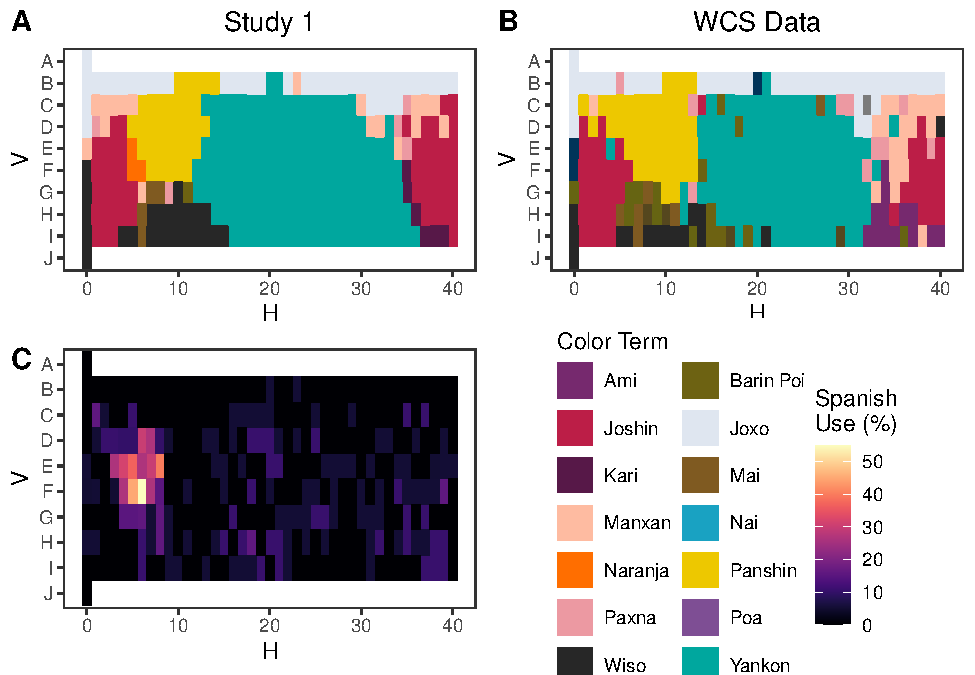
\includegraphics{amazon_color_files/figure-latex/study1-figure-1.pdf}
\caption{\label{fig:study1-figure}(A and B) Plots of the modal term given for a particular chip. Color coordinates were represented in 2-D Munsell space. Modal responses were given by SK adults during (A) the original World Color Survey and during (B) our Study 1. (C) Heat map of prevalence of Spanish-language responses during Study 1. Legends for all three subplots located in the bottom-right quadrant.}
\end{figure}

Participants used an SK-language BCT (i.e., \enquote{yankon}) to describe a median of 65\% of chips (\emph{IQR} = 53-90\%). Besides BCTs, 59\% of participants used SK-language ad hoc hue terms (i.e., \enquote{nai} or sky for blue chips) for an overall median of 6\% of chips (\emph{IQR} = 0-19\%). SK-language terms referring to saturation or luminosity of a chip, such as \enquote{manxan} (faded) were used for an overall median of 13\% of chips (\emph{IQR} = 6-20\%). Most instances (91\%) of Spanish use involved a Spanish BCT such as \enquote{rojo} (overall \emph{Mdn} = 1\%, \emph{IQR} = 0-4\%). In other words, participants responded in Spanish to label chips with basic color categories but mostly relied on SK for all other descriptor types.

\hypertarget{study-2}{%
\section{Study 2}\label{study-2}}

After generating an updated SK color term map using the responses from adult participants in Study 1, we created Study 2 to assess child participants' production and comprehension of SK color terms. Because we did not think that we could feasibly ask children across a range of ages about more than 100 color chips, we selected a subset of chips representing the prototypical instances for prominent SK terms from Study 1.

\begin{table}[tbp]

\begin{center}
\begin{threeparttable}

\caption{\label{tab:study23-demographics}Demographics of participants in Studies 2 and 3.}

\begin{tabular}{lll}
\toprule
Age Group & \multicolumn{1}{c}{n} & \multicolumn{1}{c}{Boys}\\
\midrule
\multicolumn{3}{c}{Study 1}\\
5 & 3 (5\% of overall sample) & 1\\
6 & 8 (14\%) & 3\\
7 & 12 (21\%) & 4\\
8 & 15 (26\%) & 5\\
9 & 10 (18\%) & 5\\
10 & 4 (7\%) & 2\\
11 & 5 (9\%) & 3\\
\multicolumn{3}{c}{Study 2}\\
5 & 2 (4\% of overall sample) & 1\\
6 & 2 (4\%) & 0\\
7 & 11 (24\%) & 4\\
8 & 9 (20\%) & 1\\
9 & 11 (24\%) & 4\\
10 & 8 (17\%) & 3\\
11 & 3 (7\%) & 3\\
\bottomrule
\end{tabular}

\end{threeparttable}
\end{center}

\end{table}

\hypertarget{methods-1}{%
\subsection{Methods}\label{methods-1}}

\textbf{Participants}. Fifty-seven children (23 boys) ages 5- to 11-years-old were recruited in predominantly SK neighborhoods in Yarinacocha (Nueva Era and Bena Jema) and in Bawanisho, a native community settled along the Ucayali River, more than 500 kilometers southeast of Pucallpa. Recruitment occurred either through direct contact with interested parents or through their local school. If recruited via school, consent for participation had to be given by both teacher and parent. Outside of the school environment, consent was only given by the parent.

\textbf{Materials and procedure}. Based on the findings of Study 1, we chose 8 color chips from our original set of 330 to serve as prototypical instances of major SK color terms. These color chips were blue (WCS n°1), green (n°234), red (n°245), white (n°274), yellow (n°297), black (n°312), greeny-yellow (WCS n°320), and purple (WCS n°325) (see Appendix 1). Study 2 was conducted entirely in SK and participants were explicitly instructed to give responses in SK as opposed to Spanish. In the production and comprehension tasks, children sat at a table across from the experimenter with color chips arranged between them. The production task was always performed before the comprehension task.

\textbf{Production task}. Similar to Study 1, the experimenter introduced a participant to the general procedure and the goals of the study. The experimenter would then ask: \enquote{What is the color of this chip?} As in Study 1, we used follow-up questions to elicit a BCT when the child's initial response was not a BCT. In a departure from Study 1, we were more explicit in soliciting an SK-language response. When a participant provided a Spanish-language term, the experimenter would record their response but further ask: \enquote{What is the name of this color in SK?} If a participant could not respond with an SK term, the experimenter would not ask further questions and would move forward to the next chip. As a result, some children could only produce SK non-BCTs or Spanish-language terms for particular chips.

\textbf{Comprehension task}. The comprehension task had a notably different procedure compared to the preceding production task or that of Study 1. We tested the comprehension of 9 SK color terms. The choice of these terms was based on common responses given by adult participants in Study 1. The color term prompts included BCTs: \emph{yankon} (\enquote{green/blue}), \emph{joshin} (\enquote{red}), \emph{panshin} (\enquote{yellow}), \emph{joxo} (\enquote{white/light}), \emph{wiso} (\enquote{black/dark}). We also included non-basic but prominent terms as prompts which were \emph{nai} (\enquote{blue/sky}), and \emph{barin poi} (\enquote{greenish-yellow}) and two dyads of non-basic terms \emph{pei}/\emph{xo} (\enquote{green}) and \emph{ami}/\emph{pua} (\enquote{purple}). Children sat at a table across from the experimenter with the 8 color chips of the production task displayed between them. The experimenter asked: \enquote{Can you give me the {[}\emph{color term}{]} chip?} Participants chose one of the 8 chips and their response was recorded.

Our findings from Study 1 suggested that color terms varied in their degrees of specificity. For example, \emph{wiso} best describes a narrow range of very dark to black. By contrast, \emph{yankon} could encompass blue, green, greenish-yellow, and purple; \emph{joshin} could describe red, purple, and orange; \emph{pei} or \emph{xo} to green or greenish-yellow. In cases where a term could apply for more than one chip (i.e., \emph{yankon}), the initially selected chip would be removed from the table, leaving 7 remaining chips. The experimenter would then ask: \enquote{Can you give me another {[}\emph{color term}{]} chip?} The participant would then pick another one of the 7 chips, have their response recorded, and so on. We prompted participants 4 times for \emph{yankon} and 2 times each for \emph{joshin} and \emph{pei}/\emph{xo}; every other term only received a single prompt. Due to the inherent ambiguity in term-hue pairings, accuracy for a child participant was coded based on adult responses given during Study 1. If at least 15\% of adult participants in Study 1 associated a chip with a particular term, we coded a similar term-chip pairing from a child participant as correct. Some trials could have multiple pairings, accuracy was scored as an average, rather than dichotomous. For instance, if a child correctly chose 3 out of 4 chips for the \enquote{yankon} trial, instead of 1 (correct) or 0 (incorrect) they would receive a score of 0.75.

\begin{figure}
\centering
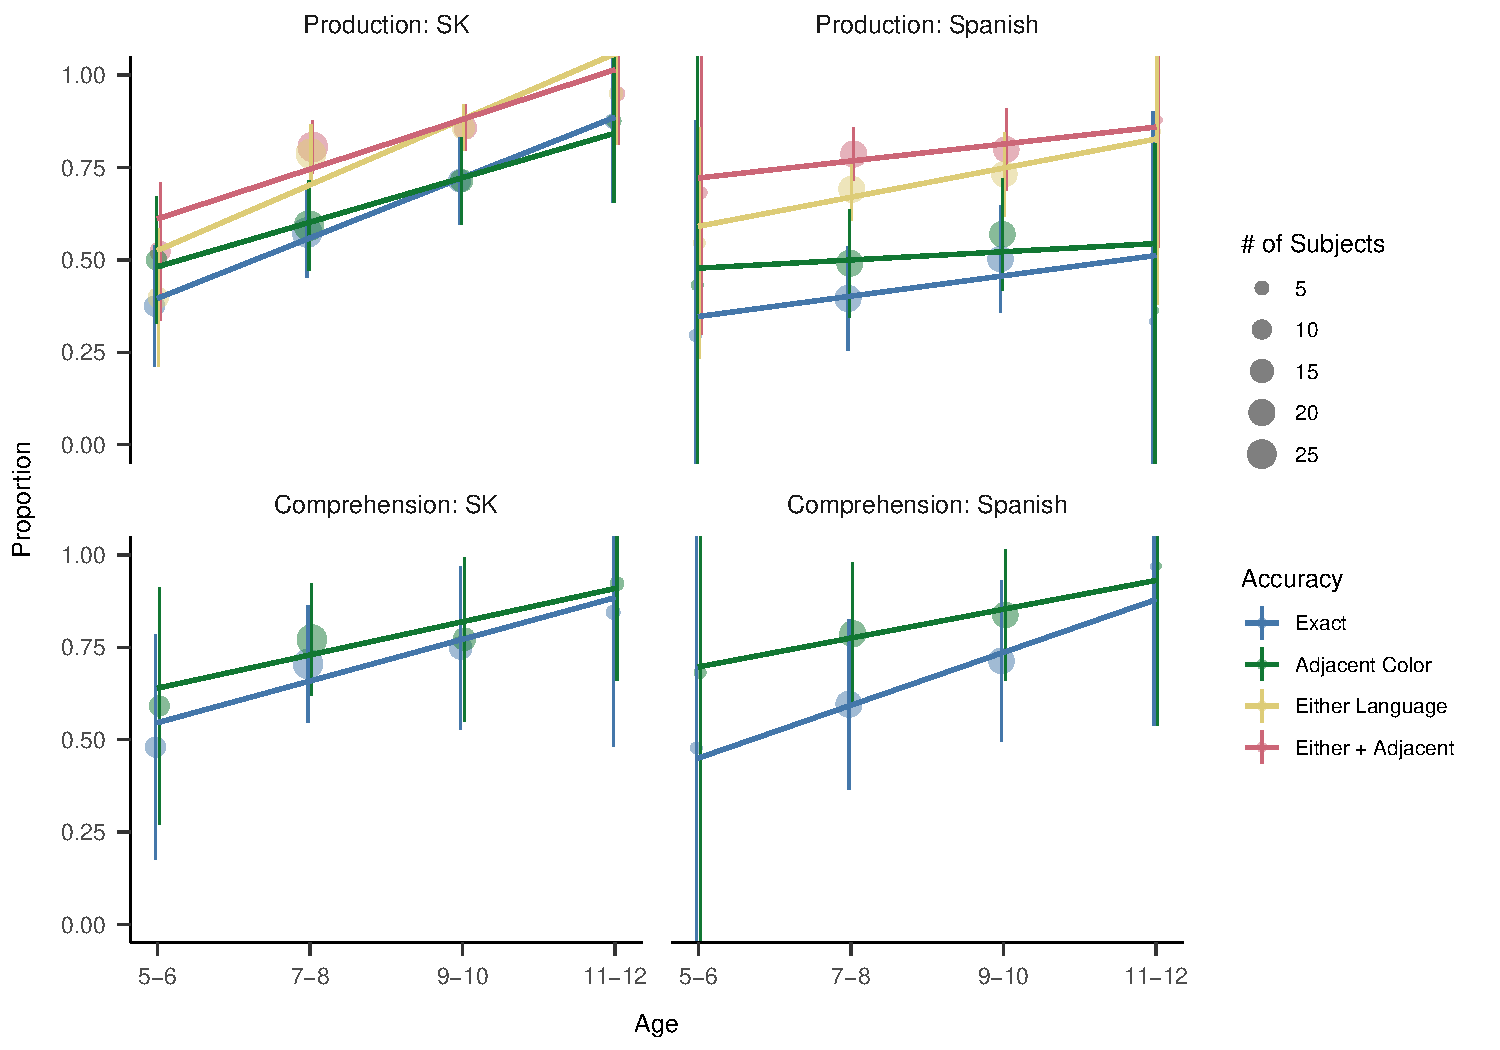
\includegraphics{amazon_color_files/figure-latex/study23-accuracy-1.pdf}
\caption{\label{fig:study23-accuracy}Proportion of accurate responses when applying different accuracy criteria, by age and study. Points show the mean for a 2-year age group (chosen arbitrarily for visualization) with 95\% confidence intervals. Lines show a loess smoothing function. Points show the mean for a 2-year age group (chosen arbitrarily for visualization) with 95\% confidence intervals.}
\end{figure}

\begin{figure}
\centering
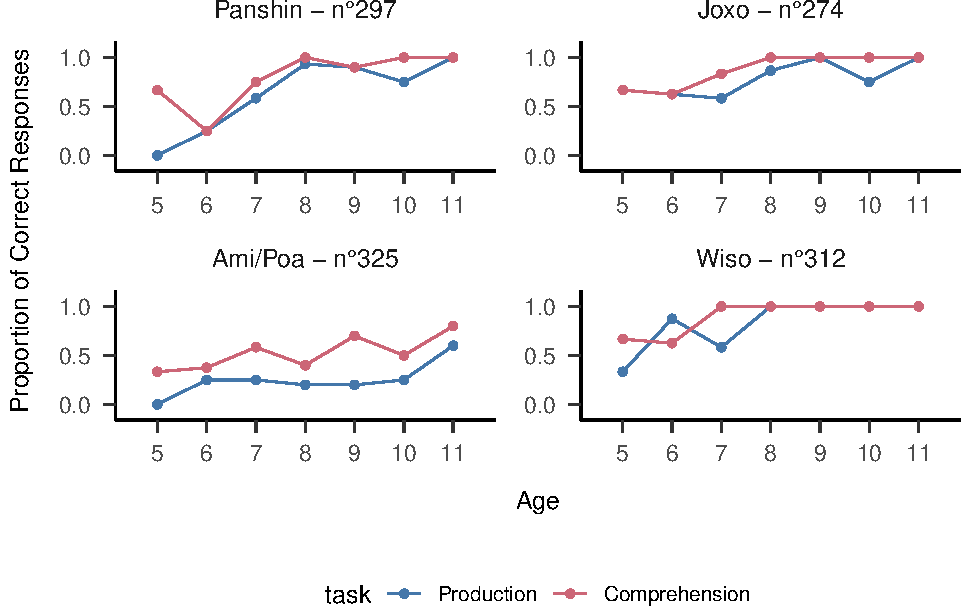
\includegraphics{amazon_color_files/figure-latex/study2-task-compare-plot-1.pdf}
\caption{\label{fig:study2-task-compare-plot}XXX Insert caption here}
\end{figure}

\hypertarget{results-and-discussion-1}{%
\subsection{Results and Discussion}\label{results-and-discussion-1}}

To confirm the existence of a developmental trajectory in SK color term knowledge, we fit generalized linear mixed-effects models (GLMMs) for both production and comprehension tasks with the following structure: accuracy of response {[}0-1{]} \textasciitilde{} age in years + (age \textbar{} prompt) + (1 \textbar{} subject). Parentheses denote random effects. Older children were more accurate in both production and comprehension compared to younger children (Figure \ref{fig:study23-accuracy}). This produced a significant developmental projection for accuracy of term-chip pairings in both production (\(\hat{\beta} = 1.05\), 95\% CI \([0.50, 1.60]\), \(z = 3.74\), \(p < .001\)) and comprehension (\(\hat{\beta} = 0.60\), 95\% CI \([0.24, 0.96]\), \(z = 3.27\), \(p = .001\)). For some term-chip pairings such as ami/pua and pei/xo, children performed failed to produce the correct term in the production task but improved significantly during the comprehension task (Figure \ref{fig:study2-task-compare-plot}). It is possible that for children's color term knowledge, comprehension precedes production. It is also possible that, given that the comprehension task always followed the production task, children were able to pick up on their errors and update their color term mapping in real-time. However, given that the experimenter did not provide feedback on accuracy during sessions, the former explanation seems more likely.

Following Frank, Braginsky, Yurovsky, and Marchman (n.d.), we used the dichotomous responses given during the production task to predict the \enquote{age of acquisition} when at least half of SK children are predicted to properly label a particular chip. First, we split responses by the prompted chip for which each participant had a single entry. For each chip, we attempted to fit a generalized linear model by robust methods (Maechler et al., 2020) with the structure \texttt{accuracy\ of\ response\ {[}0\ or\ 1{]}\ \textasciitilde{}\ age}. The coefficients for age ranged from 0.38 (odds of success multiplied by \(\exp{(\hat{\beta})}\) = 1.50 with every added year of age) to 1.35 (odds multiplied by \(\exp{(\hat{\beta})}\) = 3.80). To find age of acquisition then predicted the probability of success for the range of participant ages, 5.40- to 11.70-years-old at increments of 0.05 years, and selected the earliest age at which the accuracy crossed 0.5. Using this method, we predict that half of SK children first learn to label the \emph{joxo} chip (\enquote{white}) at 5.4 years of age. This is followed by the \emph{wiso} chip (\enquote{black}) at 5.5, the \emph{hoshin} chip (\enquote{red}) at 6.2, the \emph{panshin} chip (\enquote{yellow}) at 7.2, the \emph{yankon} chip (\enquote{green}) at 7.8, the \emph{nai} chip (\enquote{sky-blue}; \enquote{yankon} also accepted) at 9.4, and the \emph{yankon}/\emph{joshin} chip (\enquote{greenish-yellow}) at 9.5. The model for one chip (\enquote{purple}) did not predict that age of acquisition would have been met within our age range, with an estimated probability of 46\% of children successfully labelling at 11.5 years of age. It is worth noting that in Study 1, adult participants used 7 different labels for this chip (\emph{ambi}, \emph{ami}, \emph{jimi}, \emph{joshin}, \emph{kari}, \emph{morado}, and \emph{yankon}), none of which where used more than 25\% of the time. Even with the inability to predict age of acquisition for one of the 8 chips, our predictions suggest that SK children obtain color term knowledge at notably older ages compared to children in the United States (Wagner et al., 2013).

\textbf{Language switching}. Over a quarter (28\%) of all responses were given in Spanish, despite children being prompted solely in SK (i.e., labeling a panshin chip as \enquote{amarillo}). The distribution of Spanish responses was non-random, with median use in 2/8 trials (\emph{IQR} = 0-5). We failed to find a significant correlation between age and number of trials with Spanish-language responses throughout the production task (\(t(55) = -1.13\), \(p = .263\)).

\begin{table}[tbp]

\begin{center}
\begin{threeparttable}

\caption{\label{tab:study1-entropy-table}XXX Insert table title here}

\begin{tabular}{llllll}
\toprule
Chip ID & \multicolumn{1}{c}{Entropy} & \multicolumn{1}{c}{Study 2} & \multicolumn{1}{c}{Study 3} & \multicolumn{1}{c}{Shipibo term} & \multicolumn{1}{c}{Spanish term}\\
\midrule
1 & 0.71 & × &  & Nai & Celeste\\
46 & 1.72 &  & × & - & Gris\\
65 & 1.21 &  & × & - & Rosa\\
121 & 1.49 &  & × & - & Naranja\\
234 & 0.00 & × & × & Pei/Xo & Verde\\
245 & 0.21 & × & × & Joshin & Rojo\\
266 & 0.82 &  & × & - & Marron\\
274 & 0.33 & × & × & Joxo & Blanco\\
291 & 0.90 &  & × & - & Azul\\
297 & 0.21 & × & × & Panshin & Amarillo\\
312 & 0.80 & × & × & Wiso & Negro\\
320 & 1.34 & × &  & Barin Poi & Mierda sol\\
325 & 1.94 & × & × & Ami/Poa & Morado\\
\bottomrule
\end{tabular}

\end{threeparttable}
\end{center}

\end{table}

As an exploratory analysis, we attempted to quantify low naming consensus using naming entropy (following Gibson et al., 2017). We computed the naming entropy for each chip by computing the probabilities for each chip \(c\) to be named with a particular label \(l\) (\(p(l \mid c)\)) and then taking \(H(c) = - \sum{p(l\mid c) \log[p(l \mid c)]}\) (see inset entropy values by chip in Table \ref{tab:study1-entropy-table}).
To assess the hypothesis that naming entropy in adults was related to Spanish use in children, we fit a GLMM to predict likelihood of switching languages from SK to Spanish as a function of child age, entropy of the chip's naming distribution for adults in Study 1, and their interaction. This led to a model with the following structure: Different-language response {[}0 or 1{]} \textasciitilde{} age in years * prompt entropy + (1 \textbar{} subject). Despite age not being significantly correlated with overall frequency of Spanish responses, within this model, we found that older children were less likely to respond in Spanish (\(\hat{\beta} = -0.52\), 95\% CI \([-1.01, -0.03]\), \(z = -2.09\), \(p = .036\)). Children were also more likely to respond in Spanish when presented with a chip with high entropy (low naming consensus) among adult participants in Study 1 (\(\hat{\beta} = 1.54\), 95\% CI \([1.02, 2.06]\), \(z = 5.82\), \(p < .001\)). We found a positive interaction between age and entropy (\(\hat{\beta} = 0.34\), 95\% CI \([0.03, 0.66]\), \(z = 2.13\), \(p = .034\)).

\textbf{Overextensions}. One reason to use Spanish would be if children fail to recall the proper SK color term but do know the proper mapping in the Spanish. But another possibility is that children may have more imprecise representations and choose to respond with a same-language but adjacent color term (i.e., labeling a \emph{panshin}-colored chip as \enquote{joshin}). Following Wagner et al. (2013), we aggregated across color chips and examine the pattern of children's first responses, categorizing them as same-language, adjacent, and different-language. We used a GLMM to assess whether calculated word entropy and age were associated with frequency of adjacent responses using the following formula: adjacent response {[}0 or 1{]} \textasciitilde{} age in years + prompt entropy + (1 \textbar{} subject). We found that younger children were more likely to respond with SK-language but adjacent terms (\(\hat{\beta} = -1.16\), 95\% CI \([-1.96, -0.35]\), \(z = -2.81\), \(p = .005\)) but chip entropy did not have a significant factor in this strategy (\(\hat{\beta} = -1.23\), 95\% CI \([-3.00, 0.54]\), \(z = -1.36\), \(p = .173\)).

If children fail to recall the proper color term in SK, but do know the proper mapping in the Spanish color system, language-switching may be an appropriate strategy. Should they lack knowledge of the corresponding Spanish color term, they may also choose to respond with a same-language but adjacent color term. If we allow for more leniency in scoring--accepting same-language but adjacent and/or different-language but corresponding responses--we can check for more subtlety surrounding color term mapping (Figure \ref{fig:study23-accuracy}). In order to assess if changes in our scoring criteria would lead to significant changes in accuracy, we modified our original accuracy GLMM to include an interaction between age and different scoring criteria (same-language/adjacent,different-language/corresponding, and combined) which led to the following structure: accuracy of response {[}0-1{]} \textasciitilde{} age in years * scoring criteria + (age \textbar{} prompt) + (1 \textbar{} subject). We found a significant improvement in accuracy scores when we allowed different-language but corresponding responses (\(\hat{\beta} = 1.57\), 95\% CI \([1.13, 2.02]\), \(z = 6.98\), \(p < .001\)) but no significant change when allowing for same-language but adjacent responses (\(\hat{\beta} = 0.17\), 95\% CI \([-0.22, 0.56]\), \(z = 0.86\), \(p = .390\)). This increase in accuracy with language-switching strengthened with age (\(\hat{\beta} = 0.41\), 95\% CI \([0.12, 0.70]\), \(z = 2.74\), \(p = .006\)).

\hypertarget{study-3}{%
\section{Study 3}\label{study-3}}

Noting the apparent strategy of language switching seen in Study 2, we designed Study 3 as its complement. Here, we tested children's production and comprehension of Spanish color terms with a similar protocol to Study 2, albeit with a subset of chips representing prototypical colors for the Spanish color system.

\textbf{Participants}. Similar to Study 2, 46 children (16 boys) ages 5- to 11-years-old were recruited from the neighborhood of Bena Jema in Yarinacocha and from Bawanisho. Recruitment occurred either through interested parents or a local school. With consent collected from parents and, if in a school environment, teachers as well.

\textbf{Materials and procedure}. Based on Study 1 and on previous studies of Spanish color systems (XXX et al), we selected 11 color chips to serve as prototypical instances of prominent Peruvian Spanish color terms. These color chips included 6 also used during Study 2: green (n°234), red (n°245), white (n°274), yellow (n°297), black (n°312) , and purple (n°325). Five additional chips were selected: gray (WCS n°46), pink (n°65), orange (n°121), brown (n°266), and blue (n°291) (see Appendix 1). The blue chips differed between Studies 2 and 3 as we decided that the prototypical hues for \emph{yankon} and \emph{azul} differed enough to warrant the use of a different chip.

As SK children are not very fluent in Spanish (formal Spanish education occurs in adolescence), the production and comprehension tasks were both conducted in SK, and Spanish was only used for color terms (i.e., Spanish color terms were embedded within otherwise SK sentences). In both tasks, a participant would sit at a table across from the experimenter with 11 color chips in front. As in Study 2, the production task was always performed prior to the comprehension task.

\textbf{Production task}. The procedure was similar to that of both Studies 1 and 2. The experimenter would introduce a participant to the general procedure and aims of the study. Despite much of the study being conducted in SK, the experimenter would specify that participants would be expected to provide color terms in Spanish. The experimenter would then ask: \enquote{What is the color of this chip?}. If the participant responded in SK, the experimenter would record their response but further ask: \enquote{What is the name of this color in Spanish?}. If a participant responded with \enquote{I don't know} to this prompt, the experimenter would not prompt any further and would move forward to the next chip. As a result, some responses lack Spanish-language BCTs and only consist of non-basic and/or SK color terms. In total, we collected production data for 11 color chips. For each chip, the data include either one response (when children provided a Spanish basic color term in the first trial) or two or three responses (when children's initial responses were either non-basic and/or in SK).

\textbf{Comprehension task}. The procedure was similar to that of Study 2. The experimenter would ask: Can you give me the {[}\emph{color term}{]} chip? For 11 Spanish color terms. The choice of these terms was based on both previous studies examining Spanish color terms as well as responses given by adult participants in Study 1 (as some adult participants used Spanish color terms to label particular color chips). The 11 terms used as prompts were \emph{blanco} (\enquote{white}), \emph{verde} (\enquote{green}), \emph{rojo} (\enquote{red}), \emph{amarillo} (\enquote{yellow}), \emph{azul} (\enquote{blue}), \emph{negro} (\enquote{black}), \emph{naranja} (\enquote{orange}), \emph{gris} (\enquote{grey}), \emph{morado} (\enquote{purple}), \emph{marrón} (\enquote{brown}), and \emph{rosa} (\enquote{pink}). Since each color term was best instantiated by a single color chip and lacked the ambiguity seen with certain SK color terms, accuracy was graded one-to-one for term-chip pairings with less leniency compared to Study 2.

\hypertarget{results-and-discussion-2}{%
\subsection{Results and Discussion}\label{results-and-discussion-2}}

To assess age-associated changes in Spanish color term production and comprehension, we again fit GLMMs for both production and comprehension tasks with an identical structure to Study 2: accuracy of response {[}0-1{]} \textasciitilde{} age in years + (age \textbar{} prompt) + (1 \textbar{} subject). Contrasting Study 2, we found age to be a significant predictor of accuracy in the comprehension task (\(\hat{\beta} = 0.64\), 95\% CI \([0.21, 1.07]\), \(z = 2.90\), \(p = .004\)), but not in the production task (\(\hat{\beta} = 0.32\), 95\% CI \([-0.07, 0.71]\), \(z = 1.61\), \(p = .108\), see Figure \ref{fig:study23-accuracy}). Similar to Study 2, over a quarter (30\%) of all responses were given in SK, despite being prompted to respond in Spanish. There was significant variation in language-switching with some children responding solely in Spanish while others responded to upwards of 9/11 trials in SK (\emph{Mdn} = 5 trials, \emph{IQR} = 1.25-6). We found only a marginal correlation between age and accuracy (\(t(44) = 1.91\), \(p = .063\)) and no significant correlation between age and language-switching (\(t(44) = 0.44\), \(p = .663\)). Still, due to our hypothesis that older children would have more Spanish-language exposure and color term knowledge, we included age as a predictor in our GLMM assessing the effect of prompt entropy on likelihood to switch languages from Spanish to SK, similar to the one used in Study 2. With the original structure, we failed to find a significant interaction between age and prompt entropy (\(\hat{\beta} = -0.27\), 95\% CI \([-0.63, 0.09]\), \(z = -1.49\), \(p = .137\)) and removed that item, yielding the following structure: Different-language response {[}0 or 1{]} \textasciitilde{} age in years + prompt entropy + (1 \textbar{} subject). We found that participants tended to respond in SK when presented with items that had low entropy (\(\hat{\beta} = -1.49\), 95\% CI \([-2.07, -0.92]\), \(z = -5.10\), \(p < .001\)) but there was no significant effect of age (\(\hat{\beta} = -0.02\), 95\% CI \([-0.49, 0.45]\), \(z = -0.08\), \(p = .939\)). This suggests that child participants across Studies 2 and 3 preferred to respond in SK when presented with a high-consensus chip, and in Spanish with a low-consensus chip.

Similar to Study 2, we adopted alternative scoring to accommodate language-switching from Spanish to SK (different-language) but corresponding and same-language but adjacent responses. We used a GLMM identical to that of Study 2 in order to assess if changes in scoring criteria were associated with significant changes in task performance: accuracy of response {[}0-1{]} \textasciitilde{} age in years * scoring criteria + (age \textbar{} prompt) + (1 \textbar{} subject). We failed to find age as a significant predictor for accuracy even with this more lenient scoring (\(\hat{\beta} = 0.25\), 95\% CI \([-0.09, 0.58]\), \(z = 1.45\), \(p = .146\)), in concordance with earlier analyses. However, we did find that participants improved accuracy through both mapping strategies of either providing different-language but corresponding responses (\(\hat{\beta} = 1.76\), 95\% CI \([1.43, 2.09]\), \(z = 10.51\), \(p < .001\)) or same-language but adjacent responses (\(\hat{\beta} = 0.51\), 95\% CI \([0.21, 0.82]\), \(z = 3.29\), \(p = .001\)). We find frequent use of language switching in both Studies 2 and 3, but only Study 3 exhibits significant use of same-language but adjacent terms.

It is possible that early but informal Spanish language exposure can explain the discrepancies seen in Studies 2 and 3. Children may be exposed to Spanish at a young age but likely do not receive any formal Spanish education until adolescence. With limited knowledge of Spanish color terms, children may spontaneously supplement their color term knowledge with Spanish terms during SK-language Study 2 but struggle to succeed during Spanish-language Study 3. More generally, we see children relying on a mixture of strategies to communicate colors even in the absence of mastery in either language.

\hypertarget{general-discussion}{%
\section{General Discussion}\label{general-discussion}}

TO BE PASTED FROM GOOGLE DOC

In our current studies, we mapped the color vocabulary of the Shipibo-Konibo (SK) language and used these data to study the development of color vocabulary in SK children growing up in a bilingual environment. This effort parallels other efforts to use methods from language development that have typically been employed in WEIRD contexts to study populations that are under-represented in developmental science (e.g., Piantadosi et al., 2014; Fortier, Kellier, Fernández Flecha, \& Frank, n.d.).

With respect to the adult data, we found that the SK color vocabulary was relatively unchanged over the generations since the original WCS. Several interesting observations emerged, however. First, there was substantial use of Spanish terms, even though the task was conducted in SK, likely because the adults were recognizing focal colors for Spanish BCTs that have no parallel in SK (e.g., \enquote{naranja} for orange). This finding suggests an adaptive use of color vocabulary from both languages to succeed on the labeling task; future work will be required to understand whether such strategies are used in naturalistic communication as well. Second, we noted substantial use of ad-hoc color terms (including luminance terms). These terms were used more often in SK than in Spanish, supporting the idea that Amazonian languages may make greater use of ad-hoc color terms (at least in naming tasks) than Spanish speakers (e.g., Everett, 2005). Again, our data do not speak to whether this use is due to a desire to succeed on specific experimental tasks or whether it is comparable to use in naturalistic contexts. Nevertheless our findings are reminiscent of a suggestion by Levinson (2000), who noted that even purported BCTs in Yélî Dnye did not fully span hue space and were often supplemented creatively with ad-hoc terms.

When we turned to the children's data, we observed a much longer developmental trajectory for color than is observed in modern US populations. As noted by H.Bornstein (1985), however, it is a very recent development that color terms are mastered as early as they are -- one hundred years ago, US children's timeline of acquisition looked broadly similar to that observed in our study for SK children. We can only speculate as to the drivers of this historical change, but the industrialization hypothesis propounded by Gibson et al. (2017) appears to be a reasonable starting point. That is, industrialization allows for the production of identical objects that are usefully distinguished by color labeling. This communicative pressure can then lead to differentiation of color terms on a historical timescale and -- relevant to our study here -- is a likely driver of faster acquisition of color words by children. The children of one author of the current paper both learned their color terms in their second year through repeated practice with sets of manufactured plastic artifacts that varied only in hue.

Children's production and comprehension of SK and Spanish color terms was roughly comparable; there were not children who could not produce terms but had high comprehension (contra Wagner et al., 2018). Further, we did not find strong evidence for overextension in children's SK production or comprehension (with one or two exceptions). On the other hand, we did observe substantial overextension in the children's production and comprehension of Spanish color terms. This asymmetry might be due to less exposure to and/or less formal instruction in Spanish vocabulary, but this explanation is merely speculative. We did, however, observe robust evidence for competition between the SK and Spanish color systems. Children differentially used Spanish terms when there was high uncertainty for a particular color chip among adults. This finding suggests a potential route for functionally-driven language change, such that Spanish terms are borrowed -- and perhaps eventually conventionalized -- by children in cases where adult input data indicate uncertainty about the appropriate SK label.

Our data here are consistent with models of color word meaning in which color word use is driven by functional need and languages adapt by developing vocabularies that appropriately allow for communication about those needs (Gibson et al., 2017, p. @zaslavsky2018). These models have not yet been generalized to either the bilingual setting or the acquisition setting, however. Our data suggest that functional language use can cross language boundaries, inviting models that consider code switching and borrowing as part of the process of change (e.g., Myslin \& Levy, 2015).

Our work provides a descriptive comparison to studies of color naming in children learning English in the US (the focus of the majority of developmental work). Nonetheless, it has a number of limitations, some shared with this previous literature and some due to the specifics of our study and context. First, we regrettably do not have access to the kind of deep ethnographic observations that would allow us to hazard generalizations about how color terms are used in daily life among the SK communities we studied. Second, our study of development is cross-sectional and does not afford precision regarding the specific knowledge state of individual children due to the limited length of the task. Third, the limited number of color chips that we investigated means that our ability to generalize about the precision of particular color generalizations is much more limited for the children than the adults (limiting our entropy analyses). Finally, and perhaps most prominently, the kinds of tasks that we used are likely more unfamiliar to all of our participants and especially our child participants than they are to the populations being tested in investigations of WEIRD cultures (e.g., US English-learning children). While the performance of the oldest children in our studies was close to ceiling, the lower performance observed with younger children could in principle be in part a product of task unfamiliarity or other factors.

Going beyond convenience populations in experimental research with children is a new frontier for developmental science (Nielsen et al., 2017). Our work here suggests some of the benefits and challenges of this approach. On the positive, we can compare and generalize models of acquisition that are largely based on a single language and population (US English-acquiring children). At the same time, there is a paucity of resources describing language use, home environment, and cultural practices once we venture outside of WEIRD contexts. To best understand acquisition across cultures, we need to document both children's knowledge and the structure of their environments.

\newpage

\hypertarget{references}{%
\section{References}\label{references}}

\begingroup
\setlength{\parindent}{-0.5in}
\setlength{\leftskip}{0.5in}

\hypertarget{refs}{}
\leavevmode\hypertarget{ref-apicella2016}{}%
Apicella, C. L., \& Barrett, H. C. (2016). Cross-cultural evolutionary psychology. \emph{Current Opinion in Psychology}, \emph{7}, 92--97.

\leavevmode\hypertarget{ref-aragon2016}{}%
Aragón, K. (2016). Color language and color categorization. In G. Paulsen, M. Uusküla, \& J. Brindle (Eds.). Cambridge Scholars.

\leavevmode\hypertarget{ref-bartlett1977}{}%
Bartlett, E. J. (1977). \emph{Semantic organization and reference: Acquisition of two aspects of the meaning of color terms}. Biennial Meeting of the Society for Research in Child Development.

\leavevmode\hypertarget{ref-berlin1969}{}%
Berlin, B., \& Kay, P. (1969). \emph{Basic color terms: Their universality and evolution}. Berkeley, CA: University of California Press.

\leavevmode\hypertarget{ref-bornstein1976}{}%
Bornstein, M. H., Kessen, W., \& Weiskopf, S. (1976). Color vision and hue categorization in young human infants. \emph{Journal of Experimental Psychology: Human Perception and Performance}, \emph{2}(1), 115--129.

\leavevmode\hypertarget{ref-chater2010}{}%
Chater, N., \& Christiansen, M. H. (2010). Language acquisition meets language evolution. \emph{Cognitive Science}, \emph{34}(7), 1131--1157.

\leavevmode\hypertarget{ref-clark1973}{}%
Clark, E. V. (1973). Cognitive development and acquisition of language. In (pp. 65--110). Academic Press.

\leavevmode\hypertarget{ref-clark1987}{}%
Clark, E. V. (1987). Mechanisms of language acquisition. In B. MacWhinney (Ed.) (pp. 1--33). Psychology Press.

\leavevmode\hypertarget{ref-culbertson2012}{}%
Culbertson, J., Smolensky, P., \& Legendre, G. (2012). Learning biases predict a word order universal. \emph{Cognition}, \emph{122}(3), 306--329.

\leavevmode\hypertarget{ref-dobson1978}{}%
Dobson, V., \& Teller, D. Y. (1978). Visual acuity in human infants: A review and comparison of behavioral and electrophysiological studies. \emph{Vision Research}, \emph{18}(11), 1469--1483.

\leavevmode\hypertarget{ref-everett2005}{}%
Everett, D. L. (2005). Cultural constraints on grammar and cognition in pirahã another look at the design features of human language. \emph{Current Anthropology}, \emph{46}(4), 621--646.

\leavevmode\hypertarget{ref-fortierunderreview}{}%
Fortier, M., Kellier, D., Fernández Flecha, M., \& Frank, M. C. (n.d.). Ad-hoc pragmatic implicatures among shipibo-konibo children in the peruvian amazon.

\leavevmode\hypertarget{ref-frank2020}{}%
Frank, M. C., Braginsky, M., Yurovsky, D., \& Marchman, V. A. (n.d.). \emph{Variability and consistency in early language learning: The wordbank project}. Cambridge, MA: MIT Press.

\leavevmode\hypertarget{ref-frank2014}{}%
Frank, M. C., \& Goodman, N. D. (2014). Inferring word meanings by assuming that speakers are informative. \emph{Cognitive Psychology}, \emph{75}, 80--96.

\leavevmode\hypertarget{ref-franklin2005}{}%
Franklin, A., Pilling, M., \& Davies, I. (2005). The nature of infant color categorization: Evidence from eye movements on a target detection task. \emph{Journal of Experimental Child Psychology}, \emph{91}(3), 227--248.

\leavevmode\hypertarget{ref-gibson2017}{}%
Gibson, E., Futrell, R., Jara-Ettinger, J., Mahowald, K., Bergen, L., Ratnasingam, S., \ldots{} Conway, B. (2017). Color naming across languages reflects color use. \emph{Proceedings of the National Academy of Sciences}, \emph{114}(40), 10785--10790.

\leavevmode\hypertarget{ref-bornstein1985}{}%
H.Bornstein, M. (1985). On the development of color naming in young children: Data and theory. \emph{Brain and Language}, \emph{26}(1), 72--93.

\leavevmode\hypertarget{ref-henrich2010}{}%
Henrich, J., Heine, S. J., \& Norenzayan, A. (2010). The weirdest people in the world? \emph{Behavioral and Brain Sciences}, \emph{33}(2-3), 61--83.

\leavevmode\hypertarget{ref-berlin2009}{}%
Kay, P., Berlin, B., Maffin, L., Merrifield, W. R., \& Cook, R. (2009). \emph{The world color survey}. Stanford, CA: Center for the Study of Language; Information.

\leavevmode\hypertarget{ref-kitayama2007}{}%
Kitayama, S., \& Cohen, D. (2007). \emph{Handbook of cultural psychology}. Guilford Press.

\leavevmode\hypertarget{ref-kristol1980}{}%
Kristol, A. M. (1980). Color systems in southern italy: A case of regression. \emph{Language}, \emph{56}(1), 137--145.

\leavevmode\hypertarget{ref-lathrap1970}{}%
Lathrap, D. W. (1970). \emph{The upper amazon}. Thames; Hudson.

\leavevmode\hypertarget{ref-levinson2000}{}%
Levinson, S. C. (2000). Yeli dnye and the theory of basic color terms. \emph{Journal of Linguistic Anthropology}, \emph{10}(1), 3--55.

\leavevmode\hypertarget{ref-lillo2018}{}%
Lillo, J., González-Perilli, F., Prado-León, L., Melnikova, A., Álvaro, L., Collado, J. A., \& Moreira, H. (2018). Basic color terms (bcts) and categories (bccs) in three dialects of the spanish language: Interaction between cultural and universal factors. \emph{Frontiers in Psychology}, \emph{9}.

\leavevmode\hypertarget{ref-R-robustbase}{}%
Maechler, M., Rousseeuw, P., Croux, C., Todorov, V., Ruckstuhl, A., Salibian-Barrera, M., \ldots{} Anna di Palma, M. (2020). \emph{Robustbase: Basic robust statistics} (R package version 0.93-6).

\leavevmode\hypertarget{ref-monroy1989}{}%
Monroy, M., \& Custodio, S. (1989). Algunos usos de los terminos del color en el español de colombia. \emph{Thesaurus; Bogotà}, \emph{44}(2), 441.

\leavevmode\hypertarget{ref-morin1973}{}%
Morin, E. (1973). \emph{Le paradigme perdu: La nature humaine}. Éditions du Seuil.

\leavevmode\hypertarget{ref-myslin2015}{}%
Myslin, M., \& Levy, R. (2015). Code-switching and predictability of meaning in discourse. \emph{Language}, \emph{91}(4), 871--905.

\leavevmode\hypertarget{ref-nielson2017}{}%
Nielsen, M., Haun, D., Kärtner, J., \& Legare, C. H. (2017). The persistent sampling bias in developmental psychology: A call to action. \emph{Journal of Experimental Child Psychology}, \emph{162}, 31--38.

\leavevmode\hypertarget{ref-piantadosi2014}{}%
Piantadosi, S. T., Jara‐Ettinger, J., \& Gibson, E. (2014). Children's learning of number words in an indigenous farming‐foraging group. \emph{Developmental Science}, \emph{17}(4), 553--563.

\leavevmode\hypertarget{ref-regier2007}{}%
Regier, T., Kay, P., \& Khetarpal, N. (2007). Color naming reflects optimal partitions of color space. \emph{Proceedings of the National Academy of Sciences}, \emph{104}(4), 1436--1441.

\leavevmode\hypertarget{ref-sandhofer1999}{}%
Sandhofer, C. M., \& Smith, L. B. (1999). Learning color words involves learning a system of mappings. \emph{Developmental Psychology}, \emph{35}(3), 668--679.

\leavevmode\hypertarget{ref-sedivy2003}{}%
Sedivy, J. C. (2003). Pragmatic versus form-based accounts of referential contrast: Evidence for effects of informativity expectations. \emph{Journal of Psycholinguistic Research}, \emph{32}(1), 3--23.

\leavevmode\hypertarget{ref-stclair2016}{}%
St. Clair, K. (2016). \emph{The secret lives of colour}. John Murray.

\leavevmode\hypertarget{ref-surralles2016}{}%
Surrallés, A. (2016). On contrastive perception and ineffability: Assessing sensory experience without colour terms in an amazonian society. \emph{Journal of the Royal Anthropological Institute}, \emph{22}(4), 962--979.

\leavevmode\hypertarget{ref-tournon2002}{}%
Tournon, J. (2002). \emph{La merma magica: Vida e historia de los shipibo-conibo del ucayali}. Centro Amazonico de Antropologia Yaplicacion.

\leavevmode\hypertarget{ref-wagner2013}{}%
Wagner, K., Dobkins, K., \& Barner, D. (2013). Slow mapping: Color word learning as a gradual inductive process. \emph{Cognition}, \emph{127}, 307--317.

\leavevmode\hypertarget{ref-wagner2018}{}%
Wagner, K., Jergens, J., \& Barner, D. (2018). Partial color word comprehension precedes production. \emph{Language Learning and Development}, \emph{14}(4), 241--261.

\leavevmode\hypertarget{ref-yurovsky2015}{}%
Yurovsky, D., Wagner, K., Barner, D., \& Frank, M. C. (2015). Signatures of domain-general categorization mechanisms in color word learning. In \emph{Proceedings of the 37th annual conference of the cognitive science society}.

\leavevmode\hypertarget{ref-zaslavsky2018}{}%
Zaslavsky, N., Kemp, C., Tishby, N., \& Regier, T. (2018). \emph{Color naming reflects both perceptual structure and communicative need} (Vols. 1250-1255). Proceedings of the 40th Annual Conference of the Cognitive Science Society.

\endgroup


\end{document}
